\documentclass[11pt,a4paper]{article}
\usepackage{fontspec}
\setmainfont{TeX Gyre Pagella}
\newfontfamily\headfont{Inter}[UprightFont=*-ExtraBold,BoldFont=*-ExtraBold,Extension=.otf,Path=/usr/share/fonts/opentype/inter/]
\usepackage[a4paper,margin=2.3cm]{geometry}
\usepackage{graphicx,booktabs,float,caption,array,xcolor,longtable}
\usepackage{xurl}
\usepackage[hidelinks]{hyperref}
\usepackage{titlesec}
\usepackage[round]{natbib}
\usepackage{setspace}
\setstretch{1.05}
\renewcommand{\topfraction}{0.9}
\renewcommand{\bottomfraction}{0.8}
\renewcommand{\textfraction}{0.1}
\renewcommand{\floatpagefraction}{0.75}
\setlength{\parindent}{0pt}
\setlength{\parskip}{0.55em}
\titleformat{\section}{\headfont\Large}{\thesection}{0.8em}{}
\titleformat{\subsection}{\headfont\large}{\thesubsection}{0.8em}{}
\captionsetup{font=small,labelfont=bf}
\urlstyle{same}
\hypersetup{pdftitle={Where Space Rocks Land},pdfauthor={Tristan Hotham}}

\begin{document}
\begin{center}
{\Large\bfseries Where Space Rocks Land\par}
\vspace{0.4em}
{\large Falls, finds and the geography of the meteorite record:\\45,715 meteorites in the Meteoritical Bulletin, via NASA\par}
\vspace{1.2em}
{\large Tristan Hotham\par}
\vspace{0.3em}
{\small Independent researcher\\
ORCID: 0000-0003-4931-9349\\
DOI: https://doi.org/10.5281/zenodo.23847548\par}
\vspace{0.8em}
2026
\end{center}

\begin{quote}
\small
\begin{center}\textbf{Abstract}\end{center}
Meteorites reach the ground at a rate that is close to uniform over the Earth, but the catalogue of known meteorites is anything but uniform. I map the 45,715 meteorites recovered on Earth in NASA's copy of the Meteoritical Society's Meteoritical Bulletin Database (records to 2013), and separate the 1,107 witnessed falls (2.4\%) from the 44,608 finds. Finds are dominated by places where meteorites are easy to see and slow to weather: 65\% of all records come from Antarctica and 24\% from hot deserts (the Sahara 15\%, Arabia 7\%), so that ice and desert together account for 89\% of the record, almost all of it collected since 1969. Witnessed falls behave differently: none is recorded in Antarctica, where an even spread would predict about 92, and 96\% fall outside the ice and desert collection areas. Compared with an even spread over the land, Europe records 2.2 times its share of falls, Africa 0.6, South America 0.4 and Oceania 0.3; Japan, Italy, France, Germany and the United Kingdom each record more than ten times their share. Across countries, falls per unit area rise with population density (correlation on log scales 0.62). Witnessed falls grew from 17 in the 1800s to a peak of 91 in the 1930s and have since levelled at about 59 a decade. The heaviest meteorites (Hoba, Cape York, Campo del Cielo) are all iron finds, and irons make up 27\% of finds outside ice and desert against 4.4\% of falls. The map of meteorites is, above all, a map of where people have looked.

\textbf{Keywords:} meteorites; meteorite falls; Antarctic meteorites; hot desert meteorites; sampling bias; Meteoritical Bulletin; open data; mapping
\end{quote}

\section{Introduction}
Rocks from space have been falling on the Earth throughout its history, and a few of them have always been seen. The stone that fell at Ensisheim in Alsace in the 1490s was chained up in the parish church; the shower at L'Aigle in Normandy in 1803, investigated by Jean-Baptiste Biot, persuaded the scientific world that stones really do fall from the sky \citep{burke}. Since then the number of known meteorites has grown from a few hundred to tens of thousands, and the Meteoritical Society keeps the official list of names, the Meteoritical Bulletin Database \citep{metbull}.

Most of that growth did not come from new falls. It came from two discoveries about where meteorites survive and can be seen. In 1969 a Japanese expedition found nine meteorites on the bare ice near the Yamato Mountains in Antarctica \citep{yoshida}, and it soon became clear that the slow flow of the ice sheet carries meteorites to blue ice areas where wind and sublimation expose them \citep{harvey}. From the 1980s, searchers and commercial hunters in the Sahara and later in Oman found that hot deserts, with their dry, stable surfaces, preserve meteorites for tens of thousands of years and display them as dark stones on pale ground \citep{bland}.

The result is a catalogue whose map looks like a map of meteorites but is really a map of searching. This paper quantifies that, using the copy of the database that NASA publishes as open data \citep{nasa}. It asks how much of the record comes from ice and desert, how witnessed falls (which do not depend on searching) compare with an even spread over the land, and how both have changed over time. It pairs the analysis with an interactive map (\url{https://maps.tristanhotham.com/meteorite-falls/}).

\section{Data}
\textbf{Meteorites.} NASA's ``Meteorite Landings'' table, compiled from the Meteoritical Bulletin Database, gives for each meteorite its name, identifier (the Bulletin's code), whether the name is valid or relict, its class, total recovered mass, whether it was seen to fall (``Fell'') or found (``Found''), a year, and coordinates. The table has 45,716 rows and its latest records are from 2013 (11 that year); the live Bulletin has grown considerably since, so the counts here describe the catalogue to 2013. NASA's portal could not be reached from the build environment, so I used a copy mirrored on GitHub and checked it cell by cell against a second, independent GitHub mirror and a third, five-column copy. The two full copies agree on every name, class, fall status, mass and coordinate; the only differences are three archaeological finds (Havana, Ur and Wietrzno-Bobrka) that have no year in the first copy and an implausible year in the second, which I leave without a year. The data are NASA open data; I credit the Meteoritical Society and NASA throughout.

\textbf{Geography and population.} Natural Earth \citep{naturalearth} country outlines (1:10m for point in polygon and areas, 1:50m for display), with each country's land area computed as a geodesic area on the WGS84 ellipsoid, and Natural Earth's recent population estimate (POP\_EST), which I use only as a rough guide. World population for the 1960s and 2000s is from the World Bank \citep{worldbank}.

\begin{table}[tbp]\centering\small\caption{Meteorites by recovery region. `From name': placed by collection area because the record has no point.}\label{tab:reg}\begin{tabular}{lrrrrr}\toprule Region & Meteorites & Share & Finds & Falls & From name\\\midrule
Antarctica & 29,783 & 65.2\% & 29,783 & 0 & 7,684\\
Sahara & 6,754 & 14.8\% & 6,728 & 26 & 4,305\\
Arabia & 3,163 & 6.9\% & 3,154 & 9 & 0\\
Other hot deserts & 905 & 2.0\% & 902 & 3 & 1\\
Rest of the world & 3,571 & 7.8\% & 2,513 & 1,058 & 0\\
Not known & 1,539 & 3.4\% & 1,528 & 11 & 0\\
\midrule All & 45,715 & 100\% & 44,608 & 1,107 & 11,990\\
\bottomrule\end{tabular}\end{table}

\section{Methods}
\subsection{Cleaning}
Years are stored as 1 January of the year and are used as years. One record, Northwest Africa 7701, is given the year 2101 and is set to missing. One record, Meridiani Planum, was found on Mars by the Opportunity rover; it is kept in the data with a flag and left out of everything else, leaving 45,715 meteorites recovered on Earth. Coordinates that are missing (7,315 records) or exactly 0°, 0° (6,214) are treated as unknown; together 13,529 records cannot be placed on a map. Most of these are desert meteorites bought from dealers and named only for a broad area: 4,300 of the 4,499 meteorites named ``Northwest Africa'' have no point.

\subsection{Recovery regions}
Each meteorite with a point is assigned to a region: Antarctica (south of 60°S); the Sahara (a box from 15°N to 34°N and 17.5°W to 34°E); Arabia (12°N to 31°N, 35°E to 60°E); other hot deserts (the Atacama, 30°S to 18°S and 71.5°W to 68°W, and the Australian deserts including the Nullarbor, 32.5°S to 19°S and 117°E to 141°E); and the rest of the world. The boxes are deliberately simple and include some non-desert land, but very few meteorites there. Meteorites without a point take the region of their collection area, the part of the name before the number (``Yamato'' in Yamato 791197), if at least three of that area's meteorites have a point and at least 80\% of those share one region. This places 11,990 more records; 1,539 remain unknown. Present-day countries come from Natural Earth by point in polygon.

\subsection{Broad classes}
The 466 recorded classes are grouped into ordinary chondrites (H, L, LL and mixtures), carbonaceous chondrites (C groups), other chondrites (enstatite, R, K and ungrouped), achondrites (HED, ureilites, aubrites and other differentiated stones, excluding lunar and Martian), lunar, Martian, stony-irons (pallasites and mesosiderites), irons, and relict or unclassified.

\subsection{An even spread}
The flux of meteorites reaching the ground varies little over the Earth's surface; camera networks and desert surveys put it in the thousands to tens of thousands of stones above 10 g a year \citep{halliday,bland}. If every fall on land were noticed and reported, each country's share of witnessed falls would equal its share of the land area. For the 1,094 witnessed falls with a country, I compute each country's expected falls as that total times its share of the 146.8 million km\textsuperscript{2} of land in Natural Earth (Antarctica included), and report observed divided by expected. Latitude effects, and the roughly 2.4 falls into the sea for every one on land, are ignored.

\section{Results}
\subsection{Falls and finds}
Witnessed falls are 1,107 of 45,715 records (2.4\%). Table~\ref{tab:reg} and Figure~\ref{fig:reg} show where the rest come from. Antarctica has 29,783 meteorites (65\%), the Sahara 6,754 (15\%), Arabia 3,163 (7\%), most of them from Oman, and the Atacama and Australian deserts 905. The rest of the world contributes 3,571 (8\%). Among finds alone, ice and desert account for 91\%. Witnessed falls invert the picture: 96\% are in the rest of the world, 38 in the hot desert boxes, and none in Antarctica.

\begin{figure}[tbp]\centering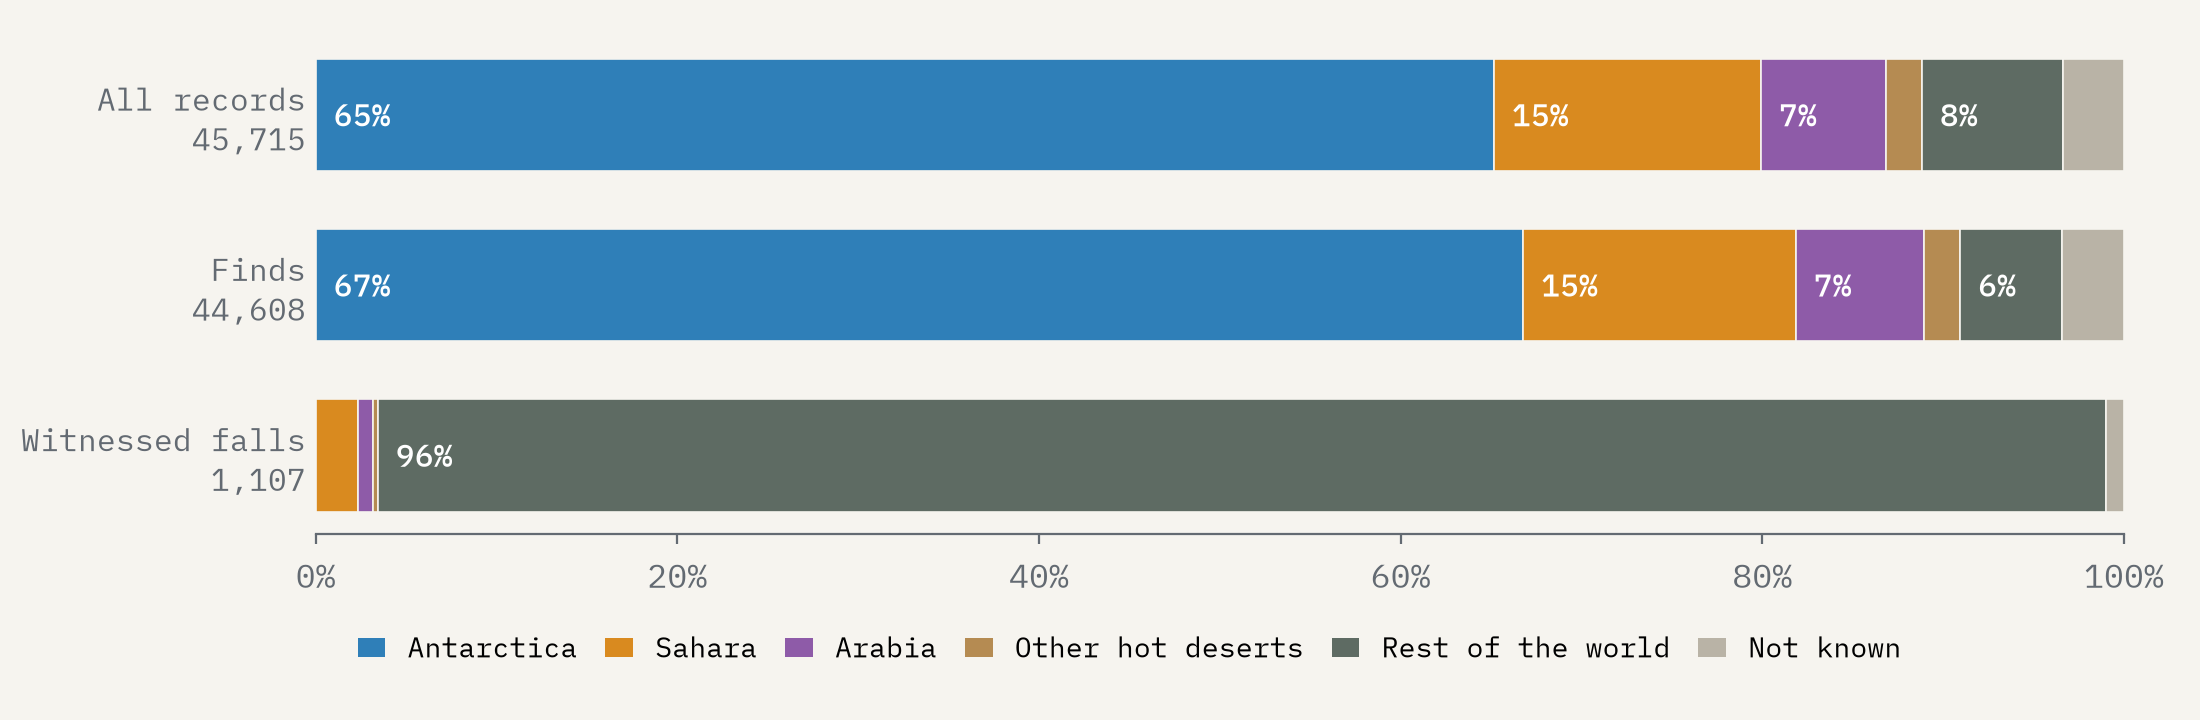
\includegraphics[width=\textwidth]{f_regions.png}
\caption{Share of meteorites by recovery region: all records, finds and witnessed falls.}\label{fig:reg}\end{figure}

\begin{figure}[tbp]\centering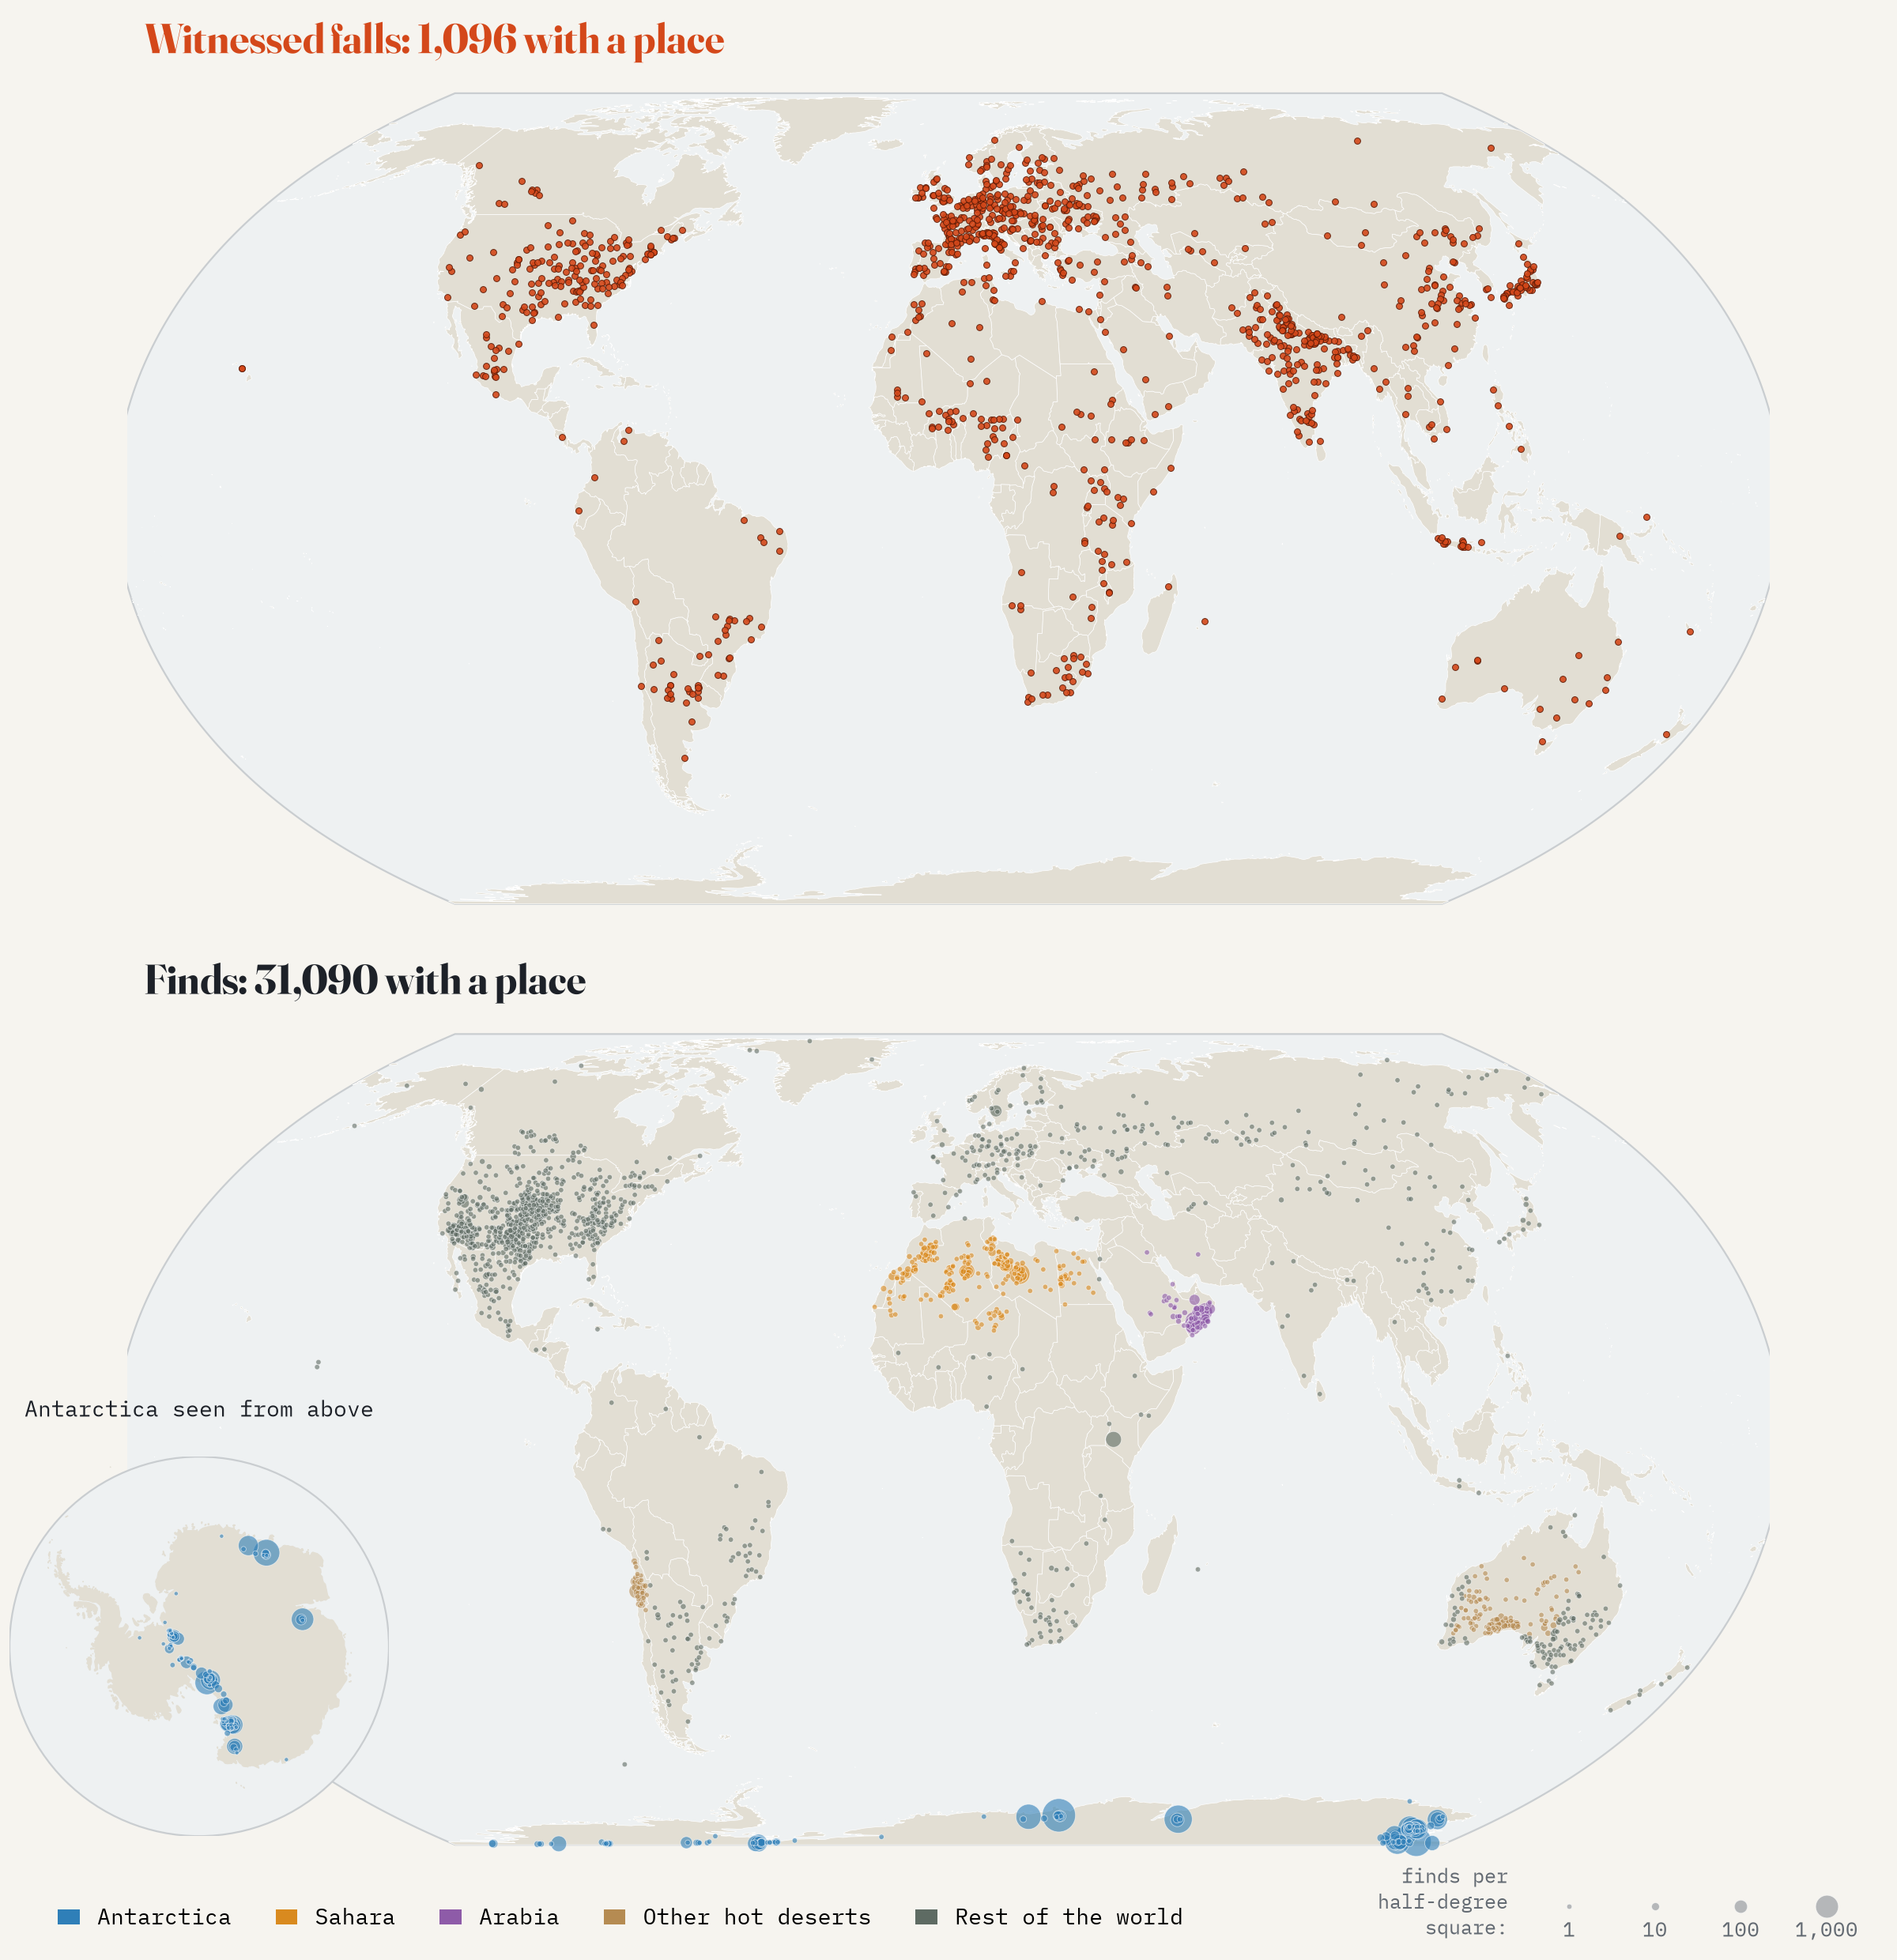
\includegraphics[width=\textwidth]{f_maps.png}
\caption{Witnessed falls (top) and finds (bottom) with a point, in the Equal Earth projection. Finds are aggregated into half-degree squares, with circle area growing with the count; the inset shows Antarctica from above.}\label{fig:maps}\end{figure}

Figure~\ref{fig:maps} maps both. The finds concentrate in a few dozen places, because a meteorite takes its name, and often its coordinates, from its collection area: the ten largest areas hold 63\% of the record (Table~\ref{tab:areas}), and thousands of Antarctic meteorites share a single point per ice field (Figure~\ref{fig:ant}). Many of these are fragments of the same fall, named separately until they are paired, so the counts overstate the number of distinct falls.

\begin{table}[tbp]\centering\small\caption{The fifteen largest collection areas (name before the number) and the first year recorded.}\label{tab:areas}\begin{tabular}{llrr}\toprule Collection area & Region & Meteorites & First year\\\midrule
Yamato & Antarctica & 7,269 & 1969\\
Northwest Africa & Sahara & 4,499 & 1970\\
Queen Alexandra Range & Antarctica & 3,444 & 1986\\
Grove Mountains & Antarctica & 2,494 & 1999\\
Elephant Moraine & Antarctica & 2,187 & 1979\\
Miller Range & Antarctica & 2,038 & 1985\\
Lewis Cliff & Antarctica & 1,870 & 1985\\
Allan Hills & Antarctica & 1,754 & 1976\\
LaPaz Icefield & Antarctica & 1,550 & 1991\\
Asuka & Antarctica & 1,509 & 1986\\
Dhofar & Arabia & 1,404 & 1998\\
Meteorite Hills & Antarctica & 1,130 & 1978\\
Dar al Gani & Sahara & 1,049 & 1995\\
MacAlpine Hills & Antarctica & 1,026 & 1987\\
Dominion Range & Antarctica & 846 & 1985\\
\bottomrule\end{tabular}\end{table}

\begin{figure}[tbp]\centering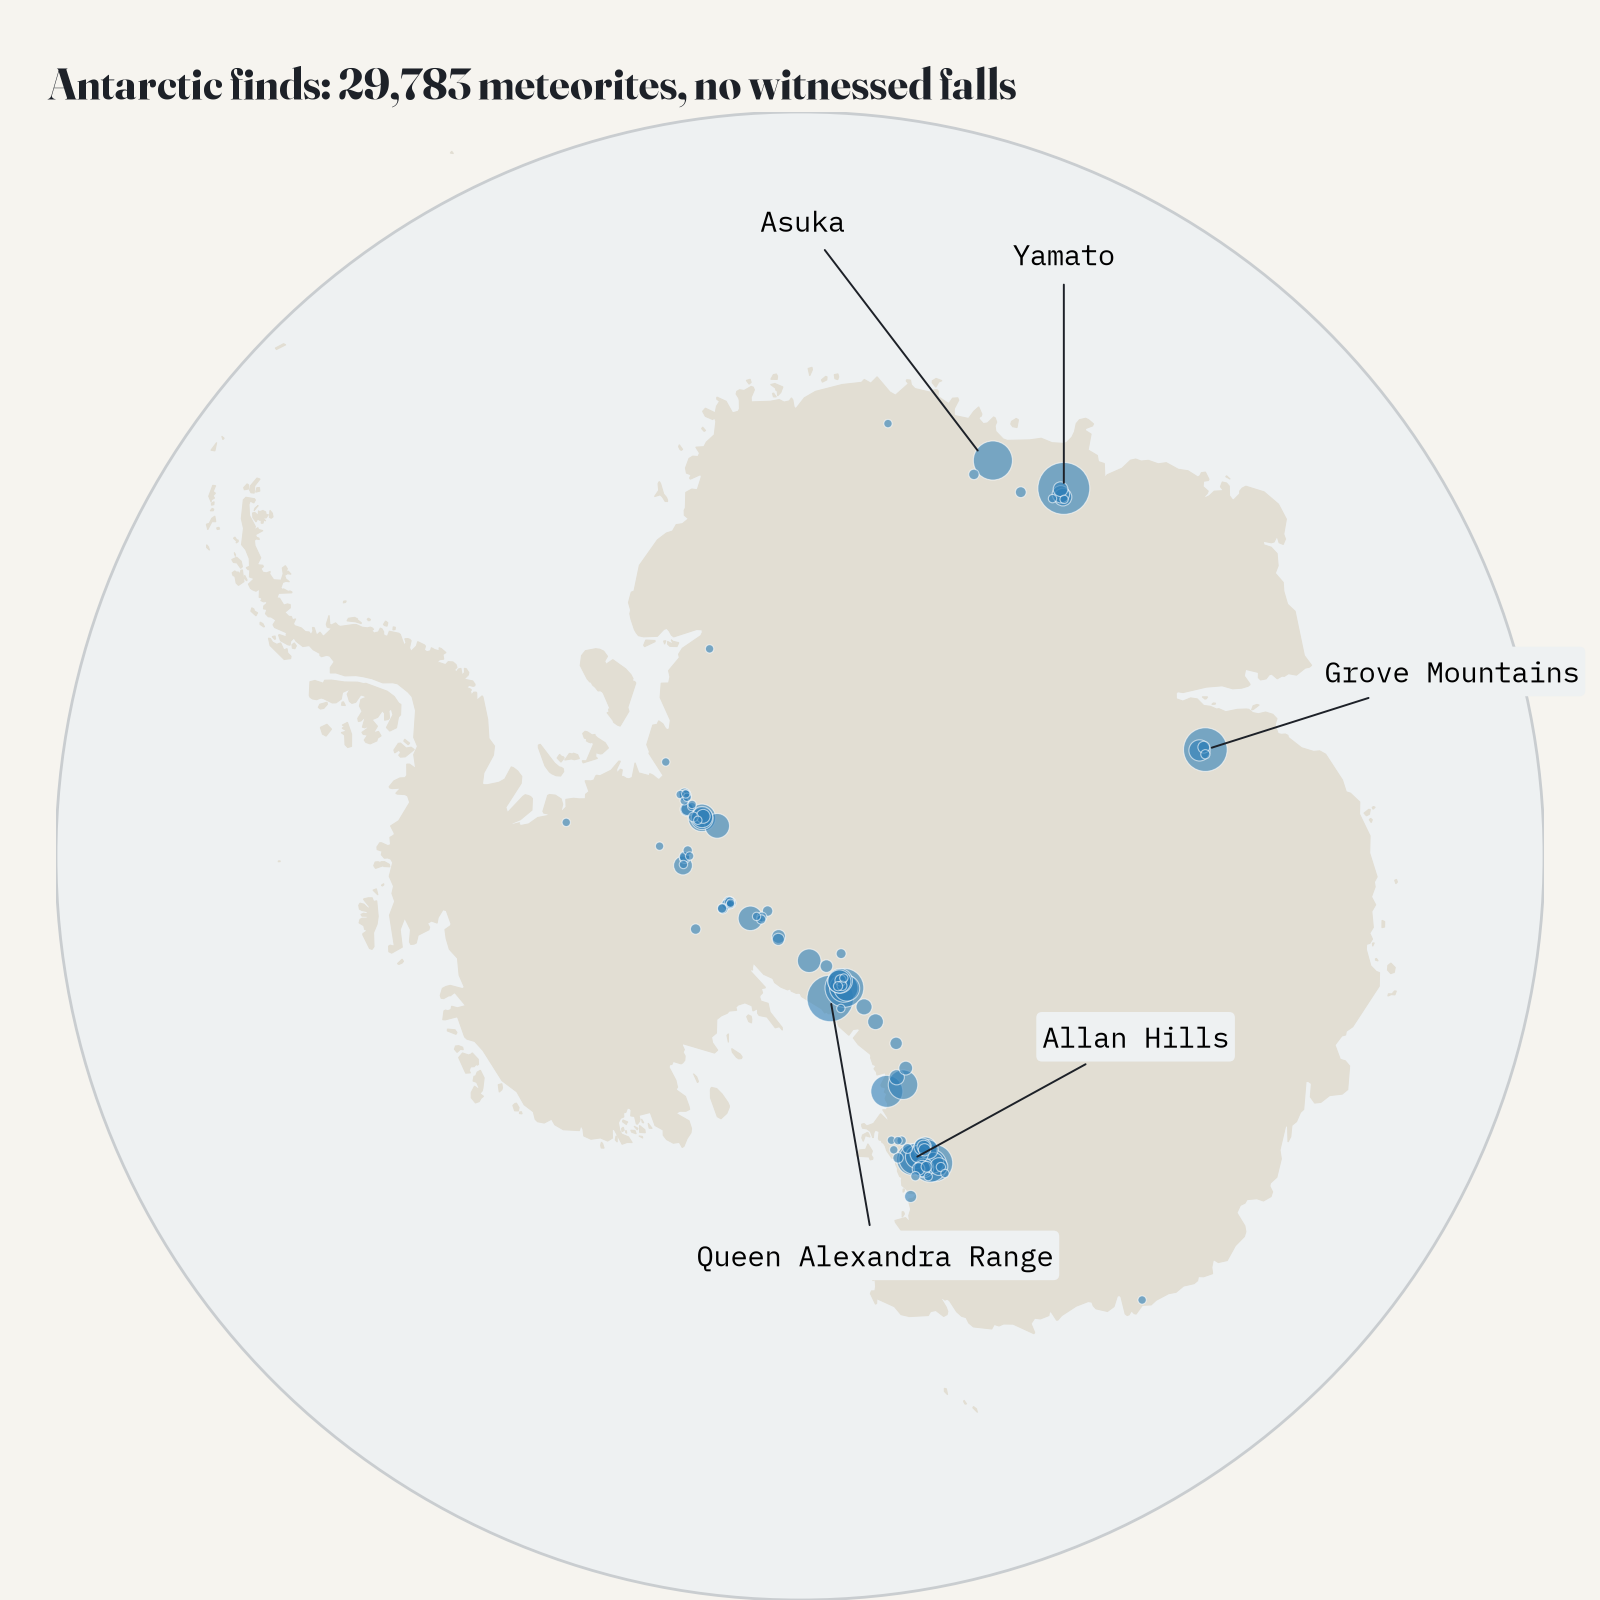
\includegraphics[width=.72\textwidth]{f_antarctica.png}
\caption{Antarctic finds by half-degree square, south polar stereographic projection. Circle area grows with the number of meteorites.}\label{fig:ant}\end{figure}

\subsection{The rush after 1969}
Before 1969 the Antarctic record held 4 meteorites besides the first, Adelie Land (1912). The Yamato discovery of 1969 (9 meteorites that year; 7,269 now carry the name) opened systematic recovery by Japanese and American programmes, and Saharan and Omani finds followed from the 1980s and 1990s. Finds per decade peak in the 2000s at 17,697, and 97\% of dated finds are from 1970 or later (Figure~\ref{fig:dec}).

\begin{figure}[tbp]\centering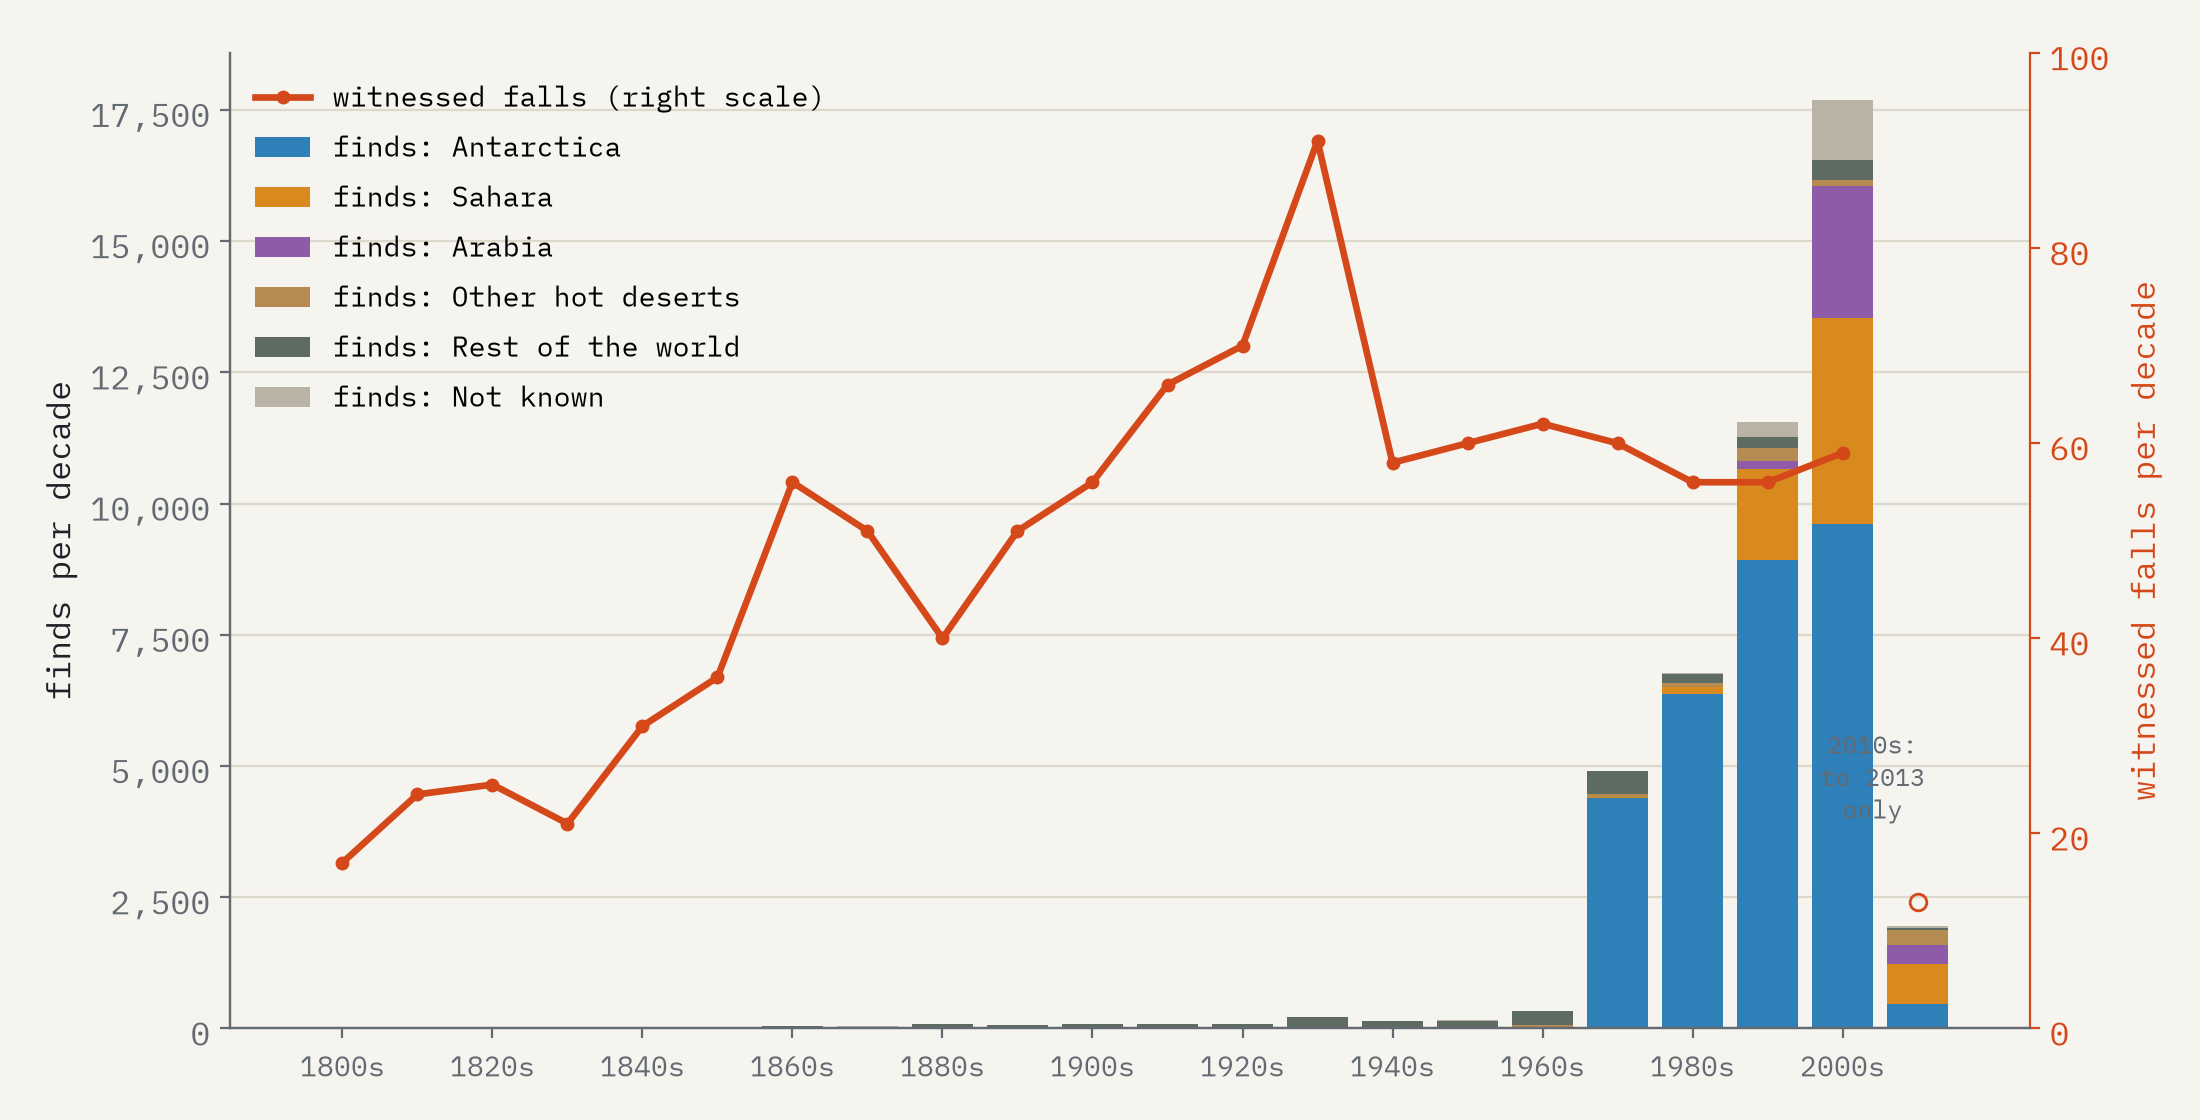
\includegraphics[width=\textwidth]{f_decades.png}
\caption{Finds per decade by recovery region (bars, left scale) and witnessed falls per decade (line, right scale). The 2010s run only to 2013 (hollow point).}\label{fig:dec}\end{figure}

Witnessed falls follow a different curve: 17 in the 1800s, 56 in the 1860s and a peak of 91 in the 1930s, after which they settle at about 59 a decade. The rise through the nineteenth century fits growing populations, literacy, newspapers and scientific interest in collecting falls. The plateau since 1950 is harder to explain with population alone: the world's population grew by 98\% between the 1960s and the 2000s, while recorded falls changed by -4.8\%. Part of the explanation may be the lag between a fall and its approval in the Bulletin, part the growth of populations in regions with fewer museums and meteorite scientists. There are 48 falls before 1800, the oldest Nogata in Japan (dated 860 in the data) and Narni in Italy (920).

\subsection{Witnessed falls against an even spread}
Table~\ref{tab:cont} and Figure~\ref{fig:cont} compare witnessed falls with an even spread by continent. Europe, with 15.7\% of the land and 9.7\% of today's population, has 34.2\% of the falls, 2.2 times its share. Asia records 1.4 times, North America 1.01, Africa 0.63, South America 0.40, Oceania 0.30 and Antarctica none of an expected 92.2.

\begin{table}[tbp]\centering\small\caption{Witnessed falls by continent against an even spread over the land. Population: Natural Earth estimate.}\label{tab:cont}\begin{tabular}{lrrrrr}\toprule Continent & Land & People & Falls & Expected & Ratio\\\midrule
Europe & 15.7\% & 9.7\% & 374 & 171.2 & 2.18\\
Asia & 21.2\% & 59.5\% & 325 & 232.3 & 1.40\\
North America & 16.5\% & 7.6\% & 183 & 180.8 & 1.01\\
Africa & 20.4\% & 17.1\% & 141 & 222.7 & 0.63\\
South America & 12.0\% & 5.6\% & 52 & 131.3 & 0.40\\
Oceania & 5.8\% & 0.6\% & 19 & 63.4 & 0.30\\
Antarctica & 8.4\% & 0.0\% & 0 & 92.2 & 0.00\\
\bottomrule\end{tabular}\end{table}

\begin{figure}[tbp]\centering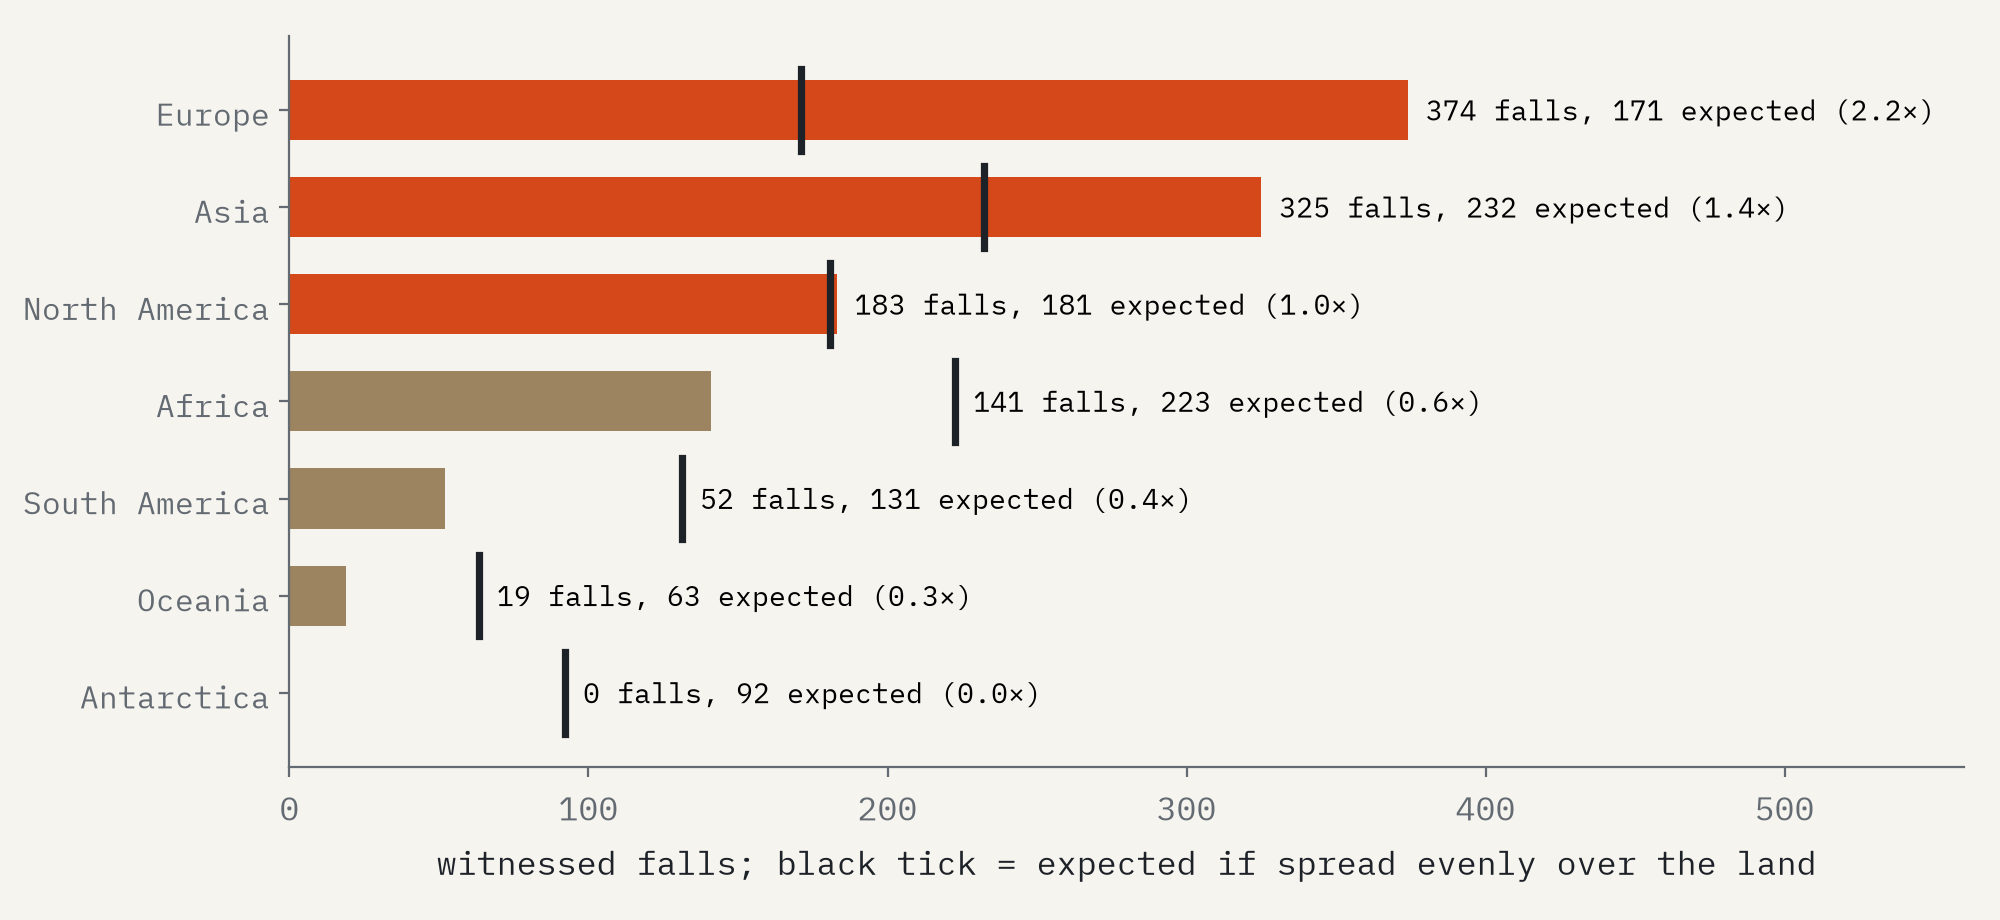
\includegraphics[width=.9\textwidth]{f_continents.png}
\caption{Witnessed falls by continent (bars) against the number expected from land area (ticks).}\label{fig:cont}\end{figure}

By country (Figure~\ref{fig:ratio}), the United States (147) and India (125) have the most falls. Relative to land area, Japan records 15.1 times its share (42 falls against 2.8 expected), Italy 13.8, France 12.9, Germany 12.0 and the United Kingdom 10.5 (19 falls); India 5.3. Large, thinly populated or dry countries record far fewer: Canada 16 of 74.1 expected, Australia 15 of 57.3, Brazil 22 of 63.1, Russia 0.39 times its share, and Libya, with 1,466 finds, 1 fall.

\begin{figure}[tbp]\centering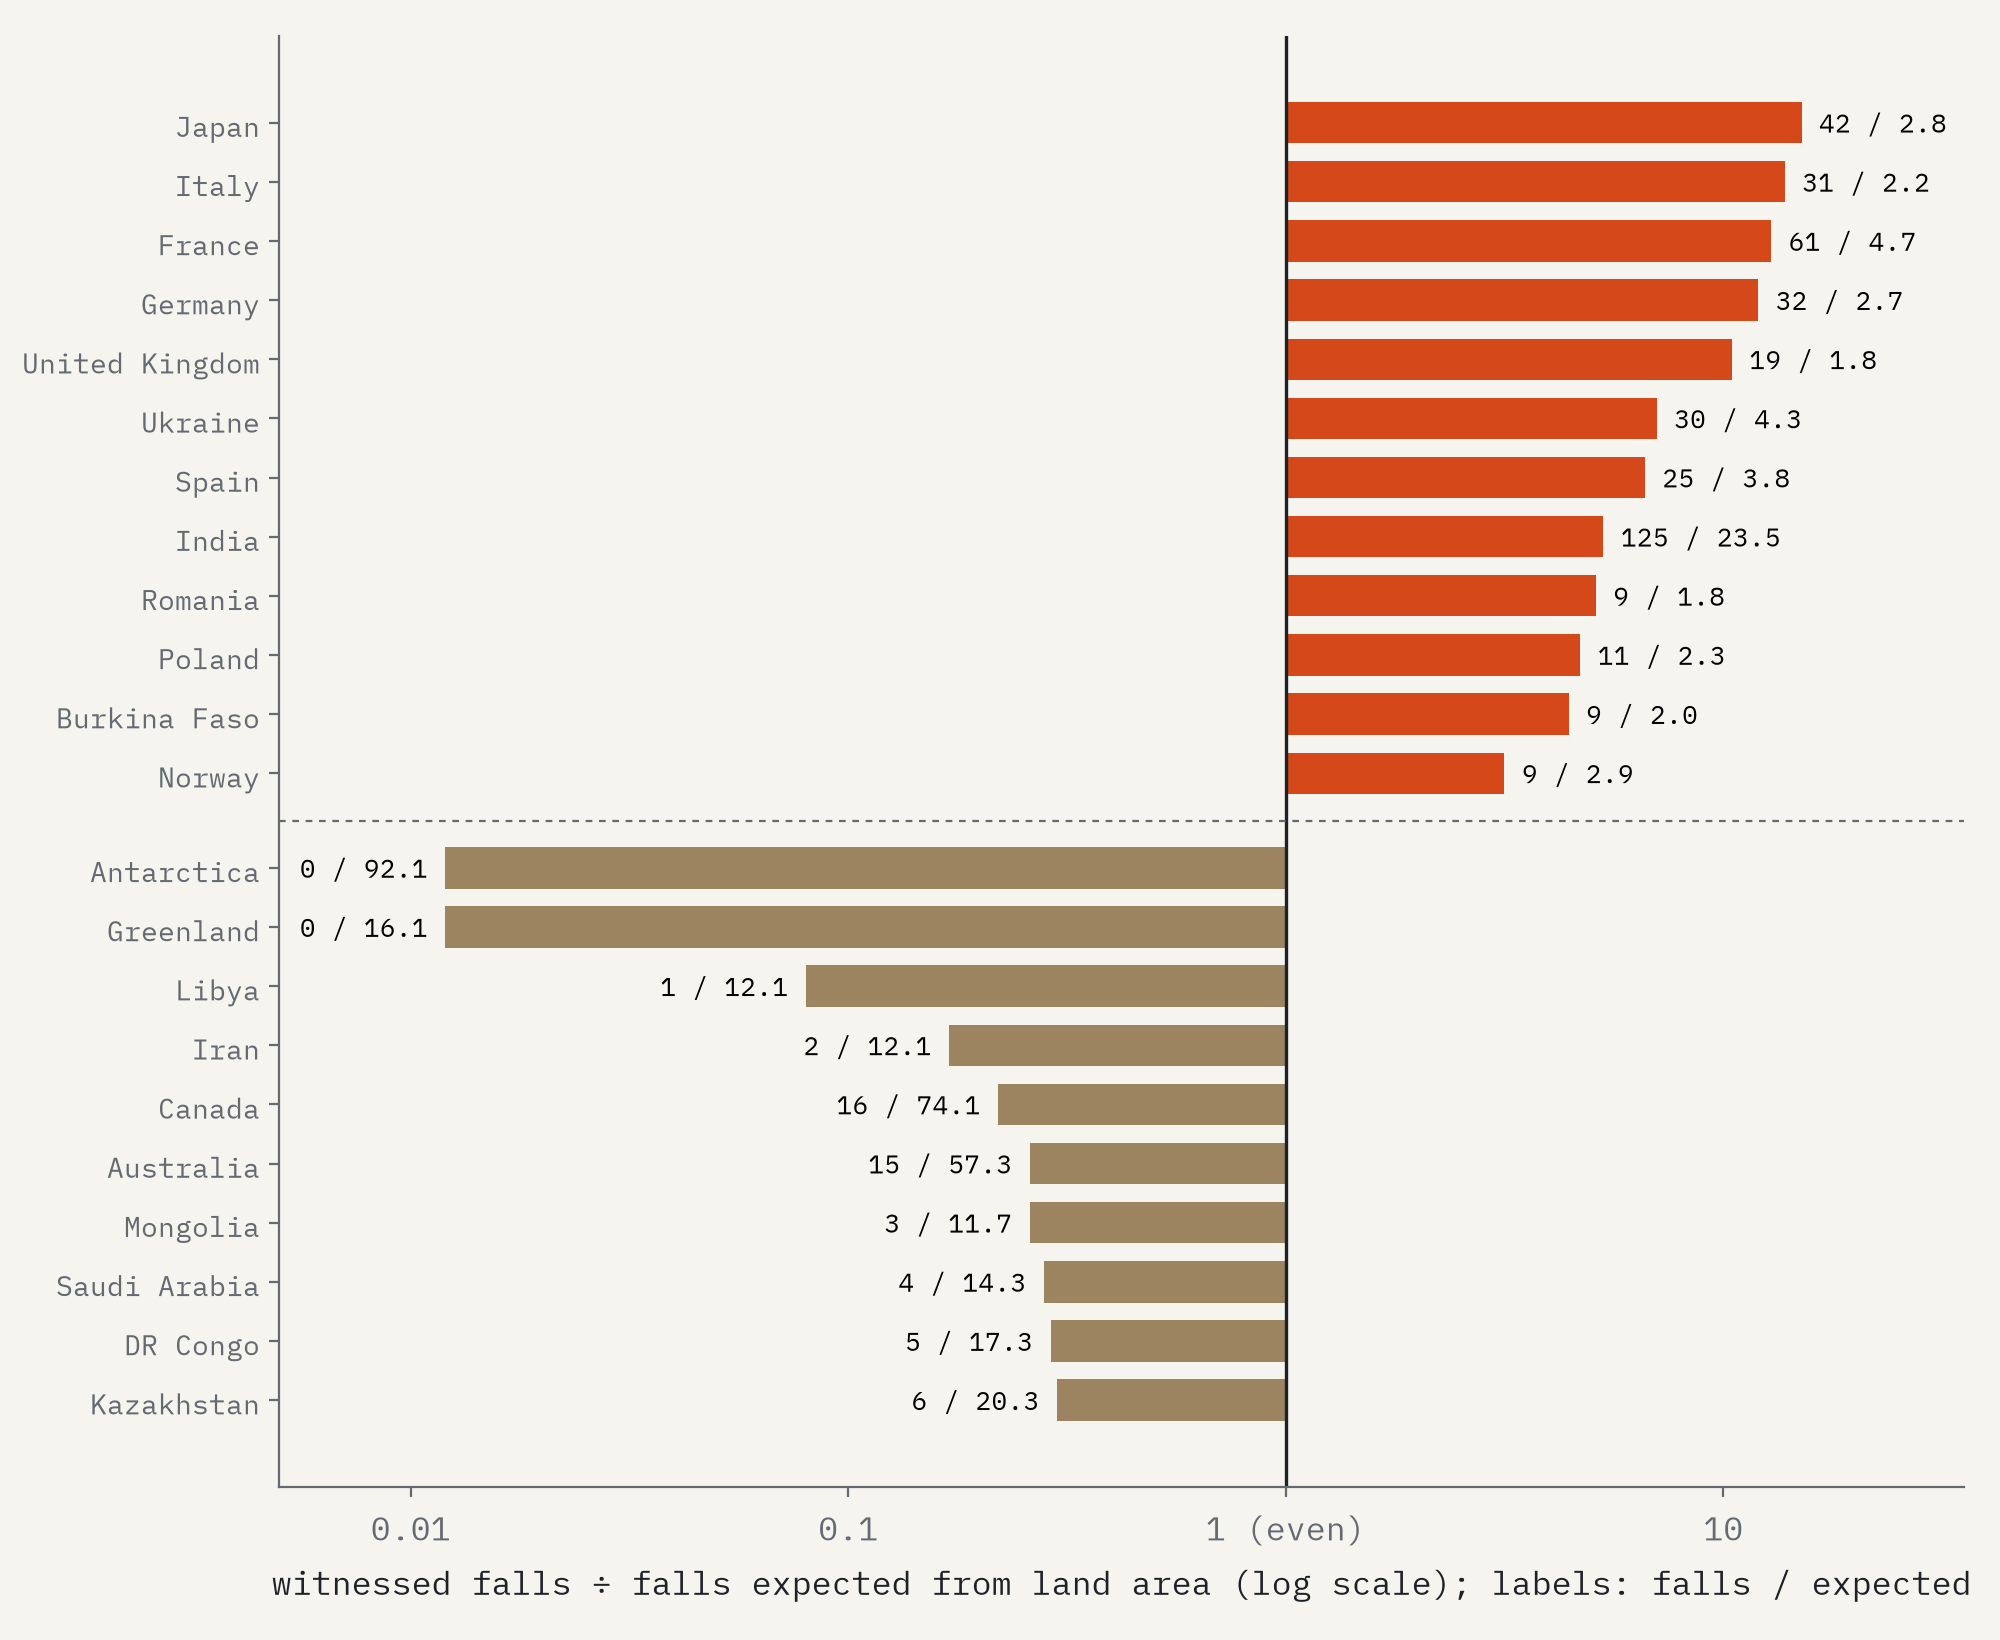
\includegraphics[width=.9\textwidth]{f_ratio.png}
\caption{Witnessed falls divided by falls expected from land area. Top: highest ratios among countries with at least 1.5 falls expected. Bottom: lowest among countries with at least 10 expected.}\label{fig:ratio}\end{figure}

\begin{table}[tbp]\centering\small\caption{The fifteen countries with most witnessed falls, with falls expected from land area.}\label{tab:countries}\begin{tabular}{lrrr}\toprule Country & Falls & Expected & Ratio\\\midrule
United States & 147 & 70.5 & 2.08\\
India & 125 & 23.5 & 5.32\\
France & 61 & 4.7 & 12.86\\
China & 58 & 69.8 & 0.83\\
Russia & 49 & 126.5 & 0.39\\
Japan & 42 & 2.8 & 15.09\\
Germany & 32 & 2.7 & 12.01\\
Italy & 31 & 2.2 & 13.81\\
Ukraine & 30 & 4.3 & 7.04\\
Spain & 25 & 3.8 & 6.62\\
Argentina & 23 & 20.7 & 1.11\\
Brazil & 22 & 63.1 & 0.35\\
Mexico & 19 & 14.6 & 1.30\\
United Kingdom & 19 & 1.8 & 10.46\\
South Africa & 18 & 9.1 & 1.98\\
\bottomrule\end{tabular}\end{table}

Population density explains much of this (Figure~\ref{fig:people}). Across the 154 countries of at least 20,000 km\textsuperscript{2}, Spearman's rank correlation between falls per km\textsuperscript{2} and people per km\textsuperscript{2} is 0.34; among the 106 with at least one fall, the Pearson correlation of the logarithms is 0.62. The scatter is wide. Europe and Japan sit above countries of similar density in South and Southeast Asia, Africa and Latin America, which points to history and institutions (long written records, a press that reported falls, museums and collectors who wanted the stones) as well as numbers of people. Population here is today's, not that at the time of each fall.

\begin{figure}[tbp]\centering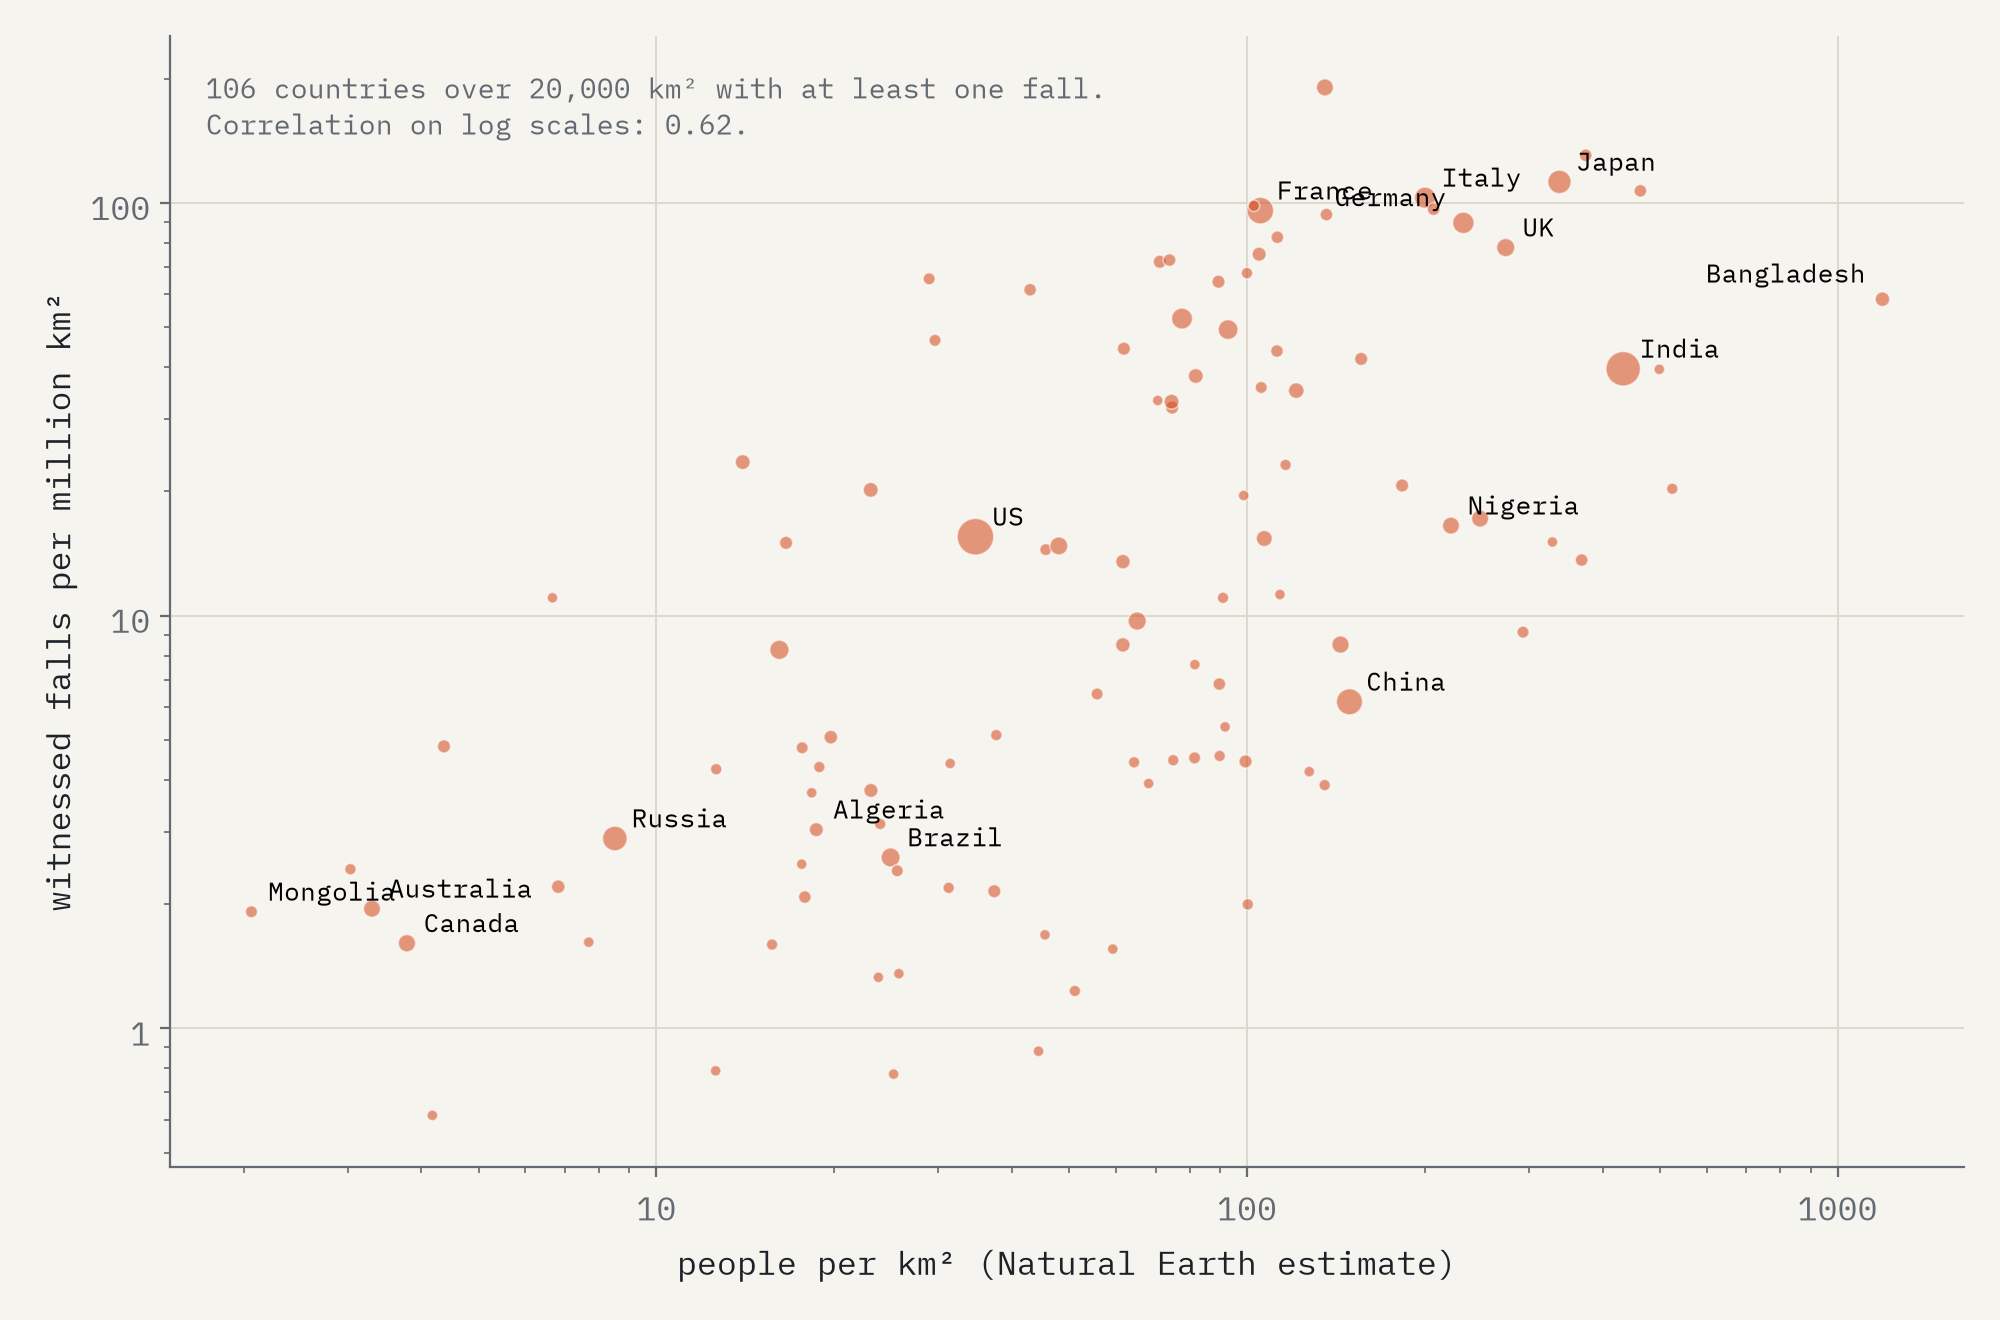
\includegraphics[width=.9\textwidth]{f_people.png}
\caption{Falls per million km\textsuperscript{2} against people per km\textsuperscript{2}, countries of at least 20,000 km\textsuperscript{2} with at least one witnessed fall. Circle size grows with the number of falls.}\label{fig:people}\end{figure}

\subsection{Mass and class}
The heaviest meteorites are all iron and almost all finds (Table~\ref{tab:heavy}): Hoba in Namibia (60.0 t), Cape York in Greenland (58.2 t, recovered in several pieces) and Campo del Cielo in Argentina (50.0 t). These three alone are 28\% of all recorded mass. The heaviest witnessed fall is Sikhote-Alin in 1947 (23.0 t), followed by Jilin (4.0 t, 1976) and Allende (2.0 t, 1969).

\begin{table}[tbp]\centering\small\caption{The twelve heaviest meteorites by total recovered mass.}\label{tab:heavy}\begin{tabular}{llrll}\toprule Meteorite & Country & Tonnes & Class & Year\\\midrule
Hoba & Namibia & 60.0 & Iron, IVB & found 1920\\
Cape York & Greenland & 58.2 & Iron, IIIAB & found 1818\\
Campo del Cielo & Argentina & 50.0 & Iron, IAB-MG & found 1575\\
Canyon Diablo & United States & 30.0 & Iron, IAB-MG & found 1891\\
Armanty & China & 28.0 & Iron, IIIE & found 1898\\
Gibeon & Namibia & 26.0 & Iron, IVA & found 1836\\
Chupaderos & Mexico & 24.3 & Iron, IIIAB & found 1852\\
Mundrabilla & Australia & 24.0 & Iron, IAB-ung & found 1911\\
Sikhote-Alin & Russia & 23.0 & Iron, IIAB & fell 1947\\
Bacubirito & Mexico & 22.0 & Iron, ungrouped & found 1863\\
Mbosi & Tanzania & 16.0 & Iron, ungrouped & found 1930\\
Willamette & United States & 15.5 & Iron, IIIAB & found 1902\\
\bottomrule\end{tabular}\end{table}

Antarctic meteorites are small: the median Antarctic find weighs 13.4 g against 235 g in the Sahara, 1,700 g for finds elsewhere and 2,800 g for witnessed falls (Figure~\ref{fig:mass}). On ice or sand a small dark stone is visible; in fields and forests only large or unusual ones are noticed.

\begin{figure}[tbp]\centering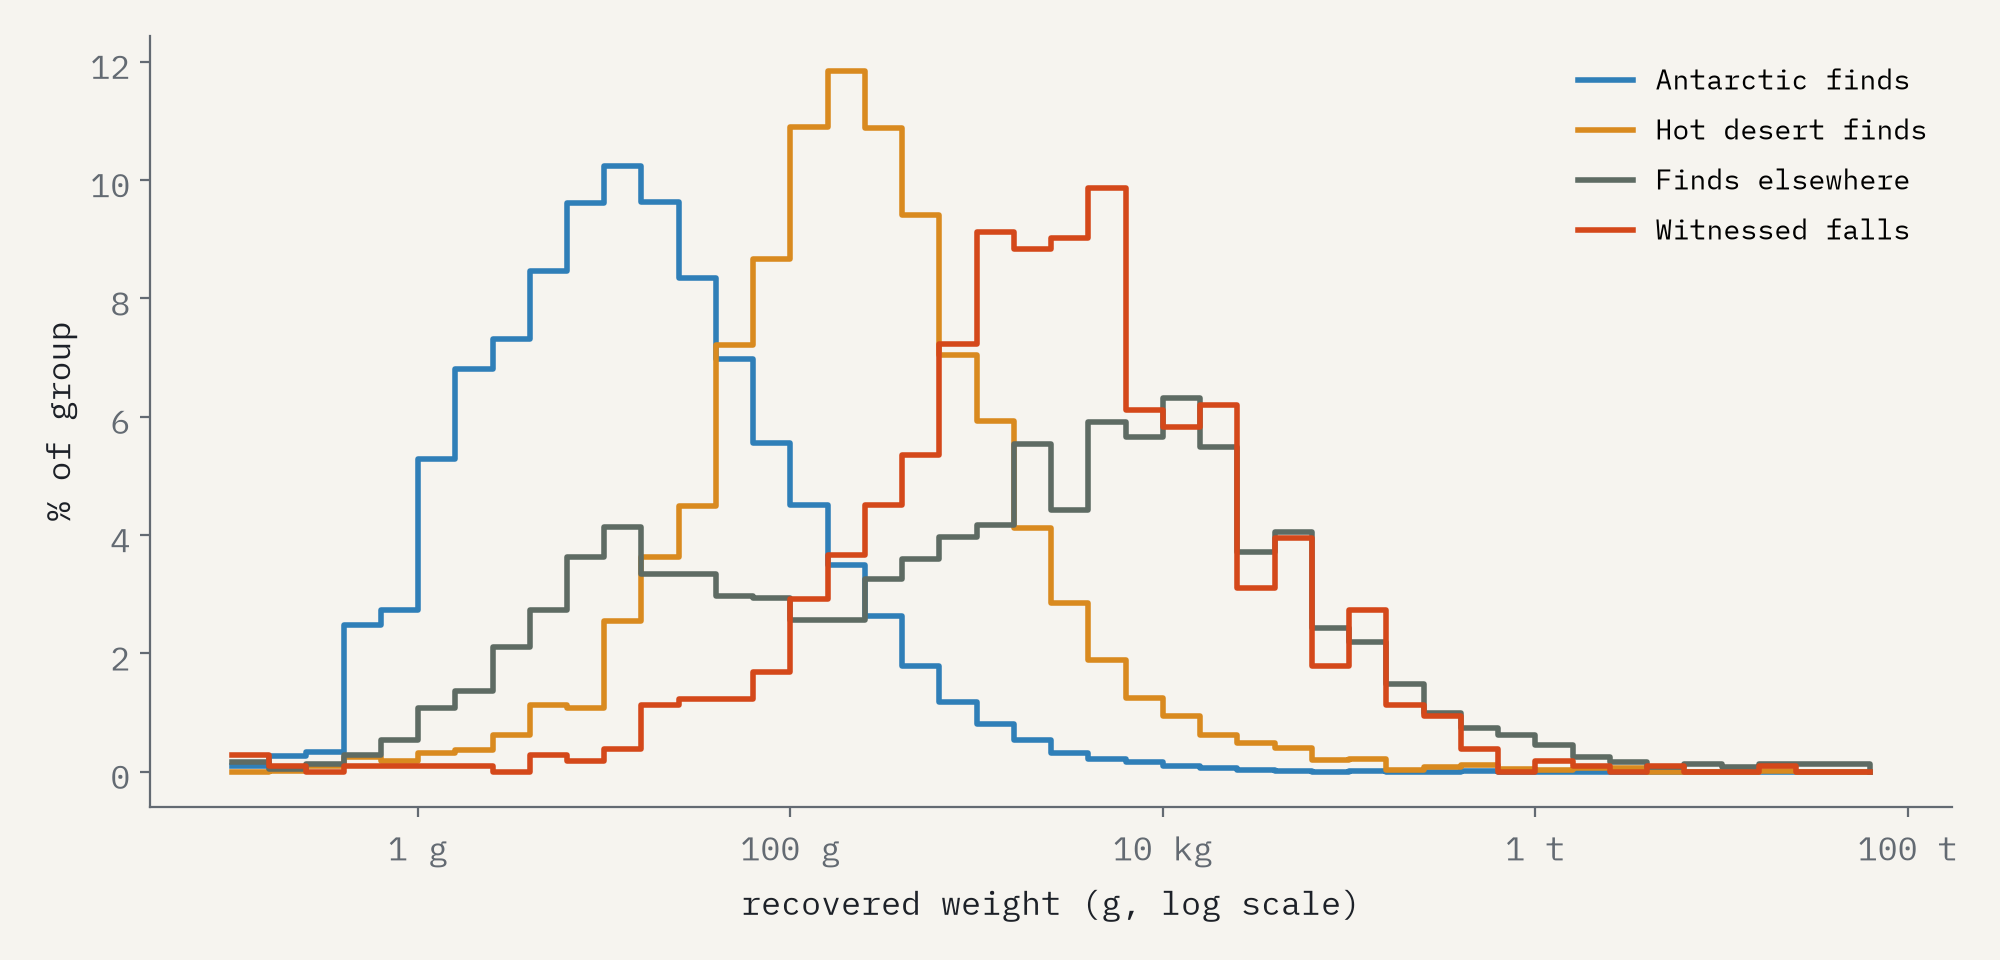
\includegraphics[width=.9\textwidth]{f_mass.png}
\caption{Distribution of recovered mass by group (meteorites with a point and a recorded mass).}\label{fig:mass}\end{figure}

The same visibility filter shows in the classes (Figure~\ref{fig:cls}). Irons are 4.4\% of witnessed falls, close to their share of what arrives, but 27.0\% of finds outside ice and desert, because they resist weathering, look unlike local rock and set off metal detectors. On ice and in deserts the mix of finds is close to that of falls and dominated by ordinary chondrites (92\% of Antarctic finds and 81\% of hot desert finds, against 77\% of falls). The rarest stones also come from ice and desert: of 119 Martian and 165 lunar meteorites, 95\% were recovered there.

\begin{figure}[tbp]\centering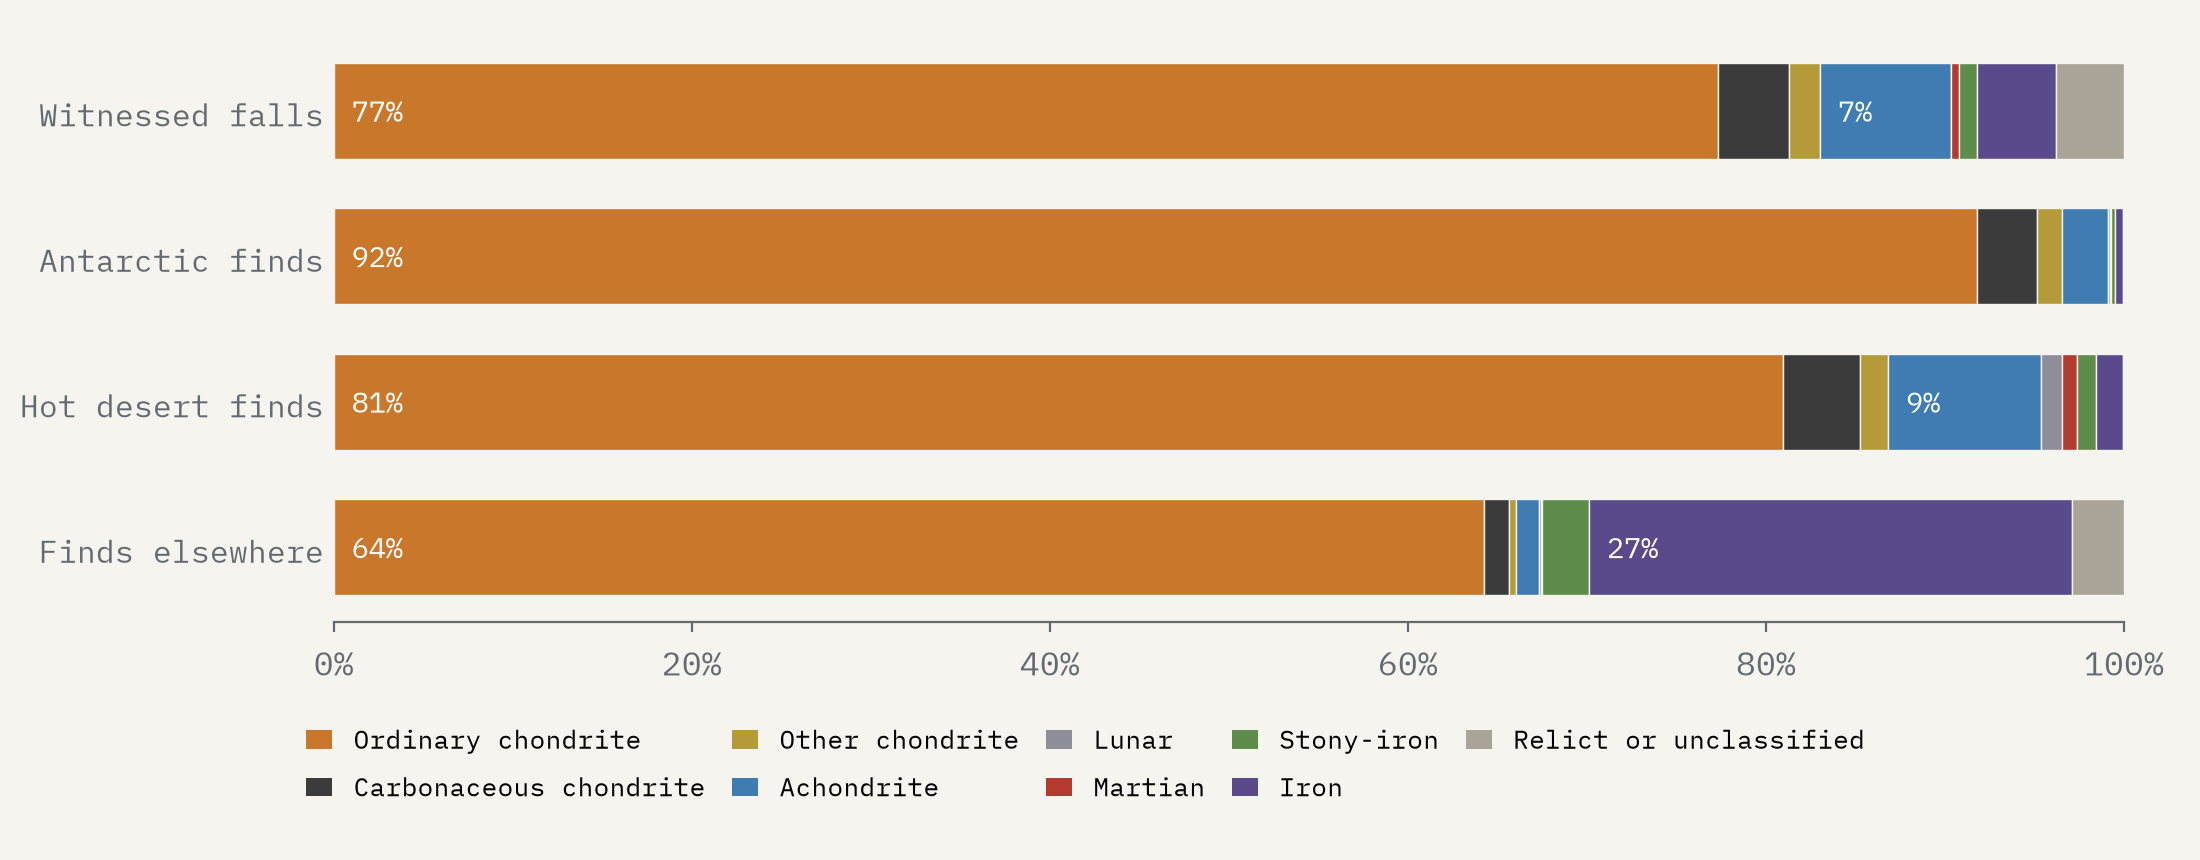
\includegraphics[width=\textwidth]{f_classes.png}
\caption{Broad class shares among witnessed falls, Antarctic finds, hot desert finds and finds elsewhere.}\label{fig:cls}\end{figure}

\section{Discussion}
None of this is new to meteoriticists, who have long known that the record is shaped by recovery \citep{harvey,bland}. What a simple map adds is a sense of scale. Almost nine in ten known meteorites come from ice or desert, and the remainder, together with the witnessed falls, are distributed much more like people than like the sky. The witnessed falls are the closest thing in the catalogue to a fair sample of what arrives, and even they are many times denser in Japan or western Europe than in Canada, Brazil or Australia.

For readers of the map, the practical lesson is to ask of any cluster whether it reflects a place where meteorites land or a place where people looked, wrote down what they saw and kept the stones.

\section{Limitations}
First, the NASA table ends in 2013 and does not include the many meteorites approved since. Second, finds have only a year of finding, not of falling. Third, many Antarctic and desert records are paired fragments of a single fall, so counts are of named meteorites, not falls. Fourth, 13,529 records have no point; I place most of them by collection area, which assumes that the area's located meteorites are representative. Fifth, the desert boxes are coarse rectangles. Sixth, population is a recent estimate and areas are present-day countries, which suits neither historical falls nor changing borders. Finally, the comparison with an even spread ignores small variations in flux with latitude.

\section{Conclusion}
The Meteoritical Society's catalogue is one of the great collaborative scientific records, and NASA's open copy makes its geography easy to see. That geography tells us more about people than about meteorites: where the ice and sand make stones easy to find, and where enough people, records and institutions turned a flash in the sky into a named stone in a museum.

\section*{Data and code availability}
The interactive map is at \url{https://maps.tristanhotham.com/meteorite-falls/}. Data and code are at \url{https://github.com/Tristan-Hotham/meteorite-falls} and archived with this paper at https://doi.org/10.5281/zenodo.23847548. Derived data are released under CC BY 4.0 and code under the MIT licence. Meteorite data: The Meteoritical Society, Meteoritical Bulletin Database, via NASA's Open Data Portal.

\section*{AI statement}
I wrote the text, with drafting and editing assistance from Claude (Anthropic), which also helped prepare the analysis code. I reviewed and checked all text and results.

\begin{thebibliography}{9}
\bibitem[Bland et al.(1996)]{bland} Bland, P. A. et al. (1996) The flux of meteorites to the Earth over the last 50,000 years. \emph{Monthly Notices of the Royal Astronomical Society}, 283, 551 to 565.
\bibitem[Burke(1986)]{burke} Burke, J. G. (1986) \emph{Cosmic Debris: Meteorites in History}. Berkeley: University of California Press.
\bibitem[Halliday et al.(1989)]{halliday} Halliday, I., Blackwell, A. T. and Griffin, A. A. (1989) The flux of meteorites on the Earth's surface. \emph{Meteoritics}, 24, 173 to 178.
\bibitem[Harvey(2003)]{harvey} Harvey, R. (2003) The origin and significance of Antarctic meteorites. \emph{Chemie der Erde}, 63, 93 to 147.
\bibitem[Meteoritical Society(2026)]{metbull} The Meteoritical Society (2026) Meteoritical Bulletin Database. \url{https://www.lpi.usra.edu/meteor/}
\bibitem[NASA(2026)]{nasa} NASA Open Data Portal (2026) Meteorite Landings (dataset gh4g-9sfh), compiled from the Meteoritical Bulletin Database. \url{https://data.nasa.gov/}
\bibitem[Natural Earth(2026)]{naturalearth} Natural Earth (2026) Admin 0 countries and populated places. Public domain. \url{https://www.naturalearthdata.com/}
\bibitem[World Bank(2026)]{worldbank} World Bank (2026) Population, total (SP.POP.TOTL). CC BY 4.0. \url{https://data.worldbank.org/}
\bibitem[Yoshida et al.(1971)]{yoshida} Yoshida, M. et al. (1971) Discovery of meteorites near Yamato Mountains, East Antarctica. \emph{Antarctic Record}, 39, 62 to 65.
\end{thebibliography}
\end{document}
